\begin{figure}[h]
  \centerline{
    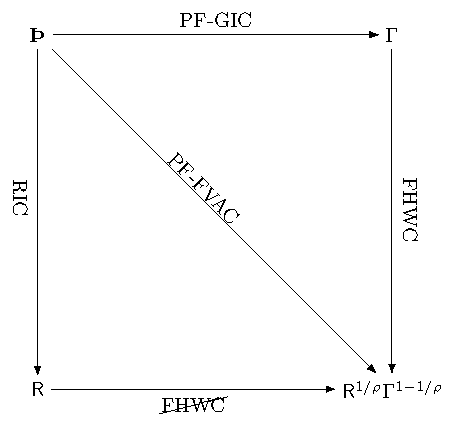
\includegraphics[width=3.5in]{\FigDir/RelatePFGICFHWCRICPFFVAC}
  }
  \caption{Relation of \PFGIC, \FHWC, \RIC, and \PFFVAC} \label{fig:RelatePFGICFHWCRICPFFVAC}
  \footnotesize{An arrowhead points to the larger of the two quantities being compared.  For example, the diagonal arrow indicates that $\Pat < \Rfree^{1/\CRRA}\PGro^{1-1/\CRRA}$, which is one way of writing the {\PFFVAC}, equation \eqref{eq:PFFVAC}}
\end{figure}
